\section{Luồng phân quyền RBAC}

Luồng RBAC mô tả cách hệ thống kiểm soát truy cập theo vai trò và quyền hạn. Đây là luồng quản trị bắt buộc vì hệ thống đồng thời có người dùng cuối, quản trị viên nội dung và quản trị viên hệ thống; mỗi nhóm chỉ được thực hiện đúng các thao tác được cấp phép.

\begin{figure}[H]
    \centering
    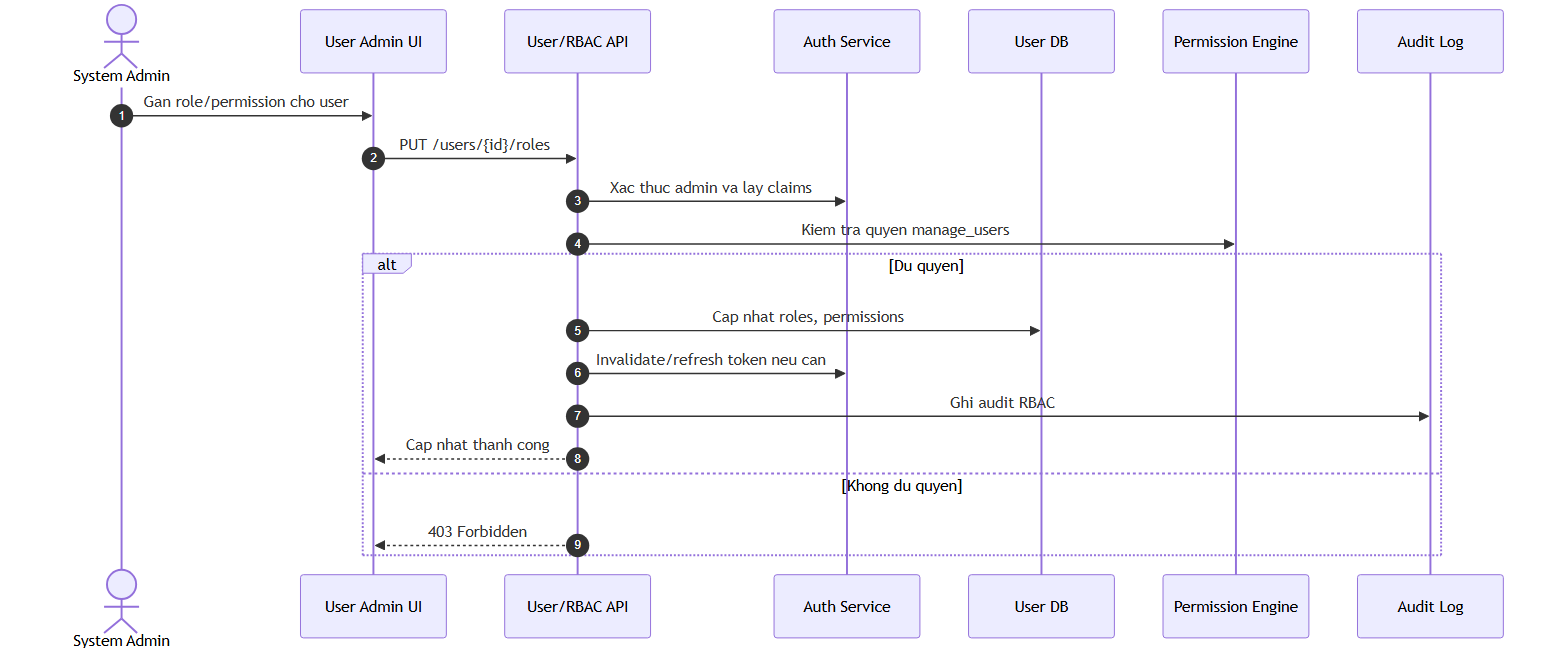
\includegraphics[width=\textwidth]{content/source/mermaid_sequence/seq_09.png}
    \caption{Luồng phân quyền RBAC}
\end{figure}

Theo sequence, quản trị viên tạo vai trò, định nghĩa quyền cho vai trò, gán vai trò vào người dùng và để frontend áp dụng kiểm tra quyền trước khi hiển thị hoặc kích hoạt chức năng. Khi người dùng gọi API, backend tiếp tục xác thực token, kiểm tra quyền trên tài nguyên và chỉ cho phép thao tác nếu vai trò tương ứng đáp ứng điều kiện. Cách thiết kế này bảo đảm vừa có lớp chặn ở giao diện, vừa có lớp kiểm soát thực sự ở backend.
